% !TeX root = ../../master_thesis.tex

\section{Satisfaction with current state of front-office}

As it was previously analyzed, chat-bot solution may require both a lot of time and a lot of resources to develop.
Intuitively, we may expect mentioned ML\&AI-based chat-bots to be an ideal, automated solution for cost decrease and effective customer support.
Unfortunately, banking clients may have subjectively negative opinion on existing rule-based chat-bots, which are usually considered as an avantguarde of customer support, but may not help properly client needs.

Therefore, survey was conducted in order to determine current level of satisfaction with front-office.
In entire survey 278 respondents were involved.

First question was to build an age portrait. 
Age answers were divided in three categories based on generation experience with dialog interfaces.
First group lower limit of 18 years was chosen due to socially acceptable age of responsibility.
First group upper limit of 32 years was chosen as dialog interfaces became most viable nearly 15 years ago, resulting in experienced users of dialog interfaces.
Second group upper limit was chosen based on a socially acceptable middle-age medium. 
It is possible to observe dominance of young generation among respondents.

\begin{figure}
    \centering
    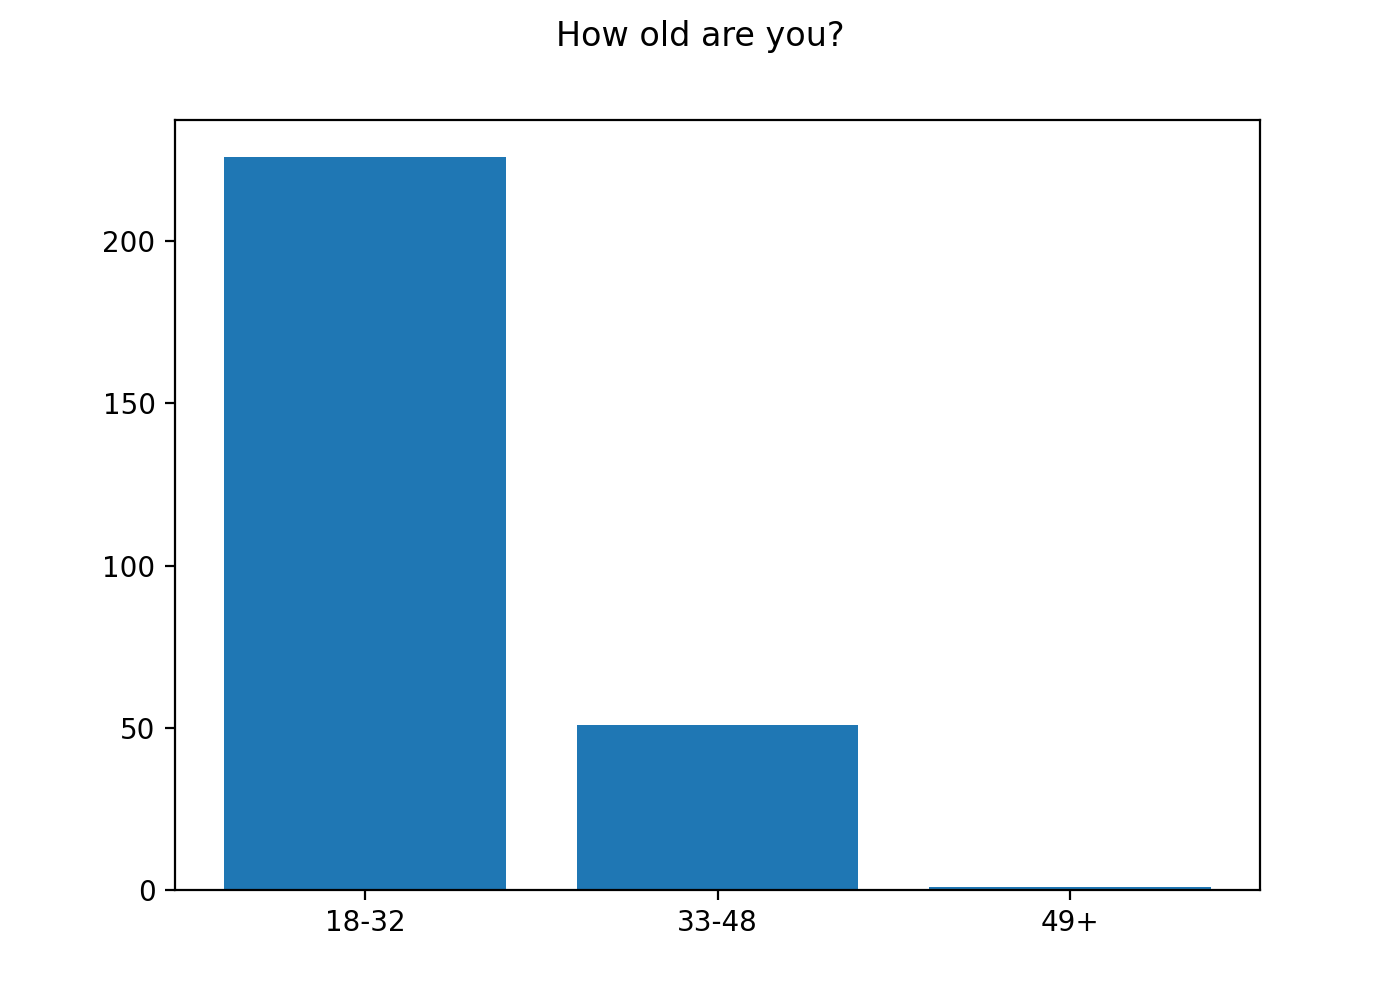
\includegraphics[width=0.6\textwidth,height=\textheight,keepaspectratio]{survey/1_how_old_are_you?.png}
    \caption{Ages of respondents}
    \medskip
    \footnotesize\textit{Source:} Own study.
\end{figure}

On the other hand, second question had shown high levels experience of banking interactions among respondents, as more than a half of respondents used services of 2 or more banks for the last year.

\begin{figure}
    \centering
    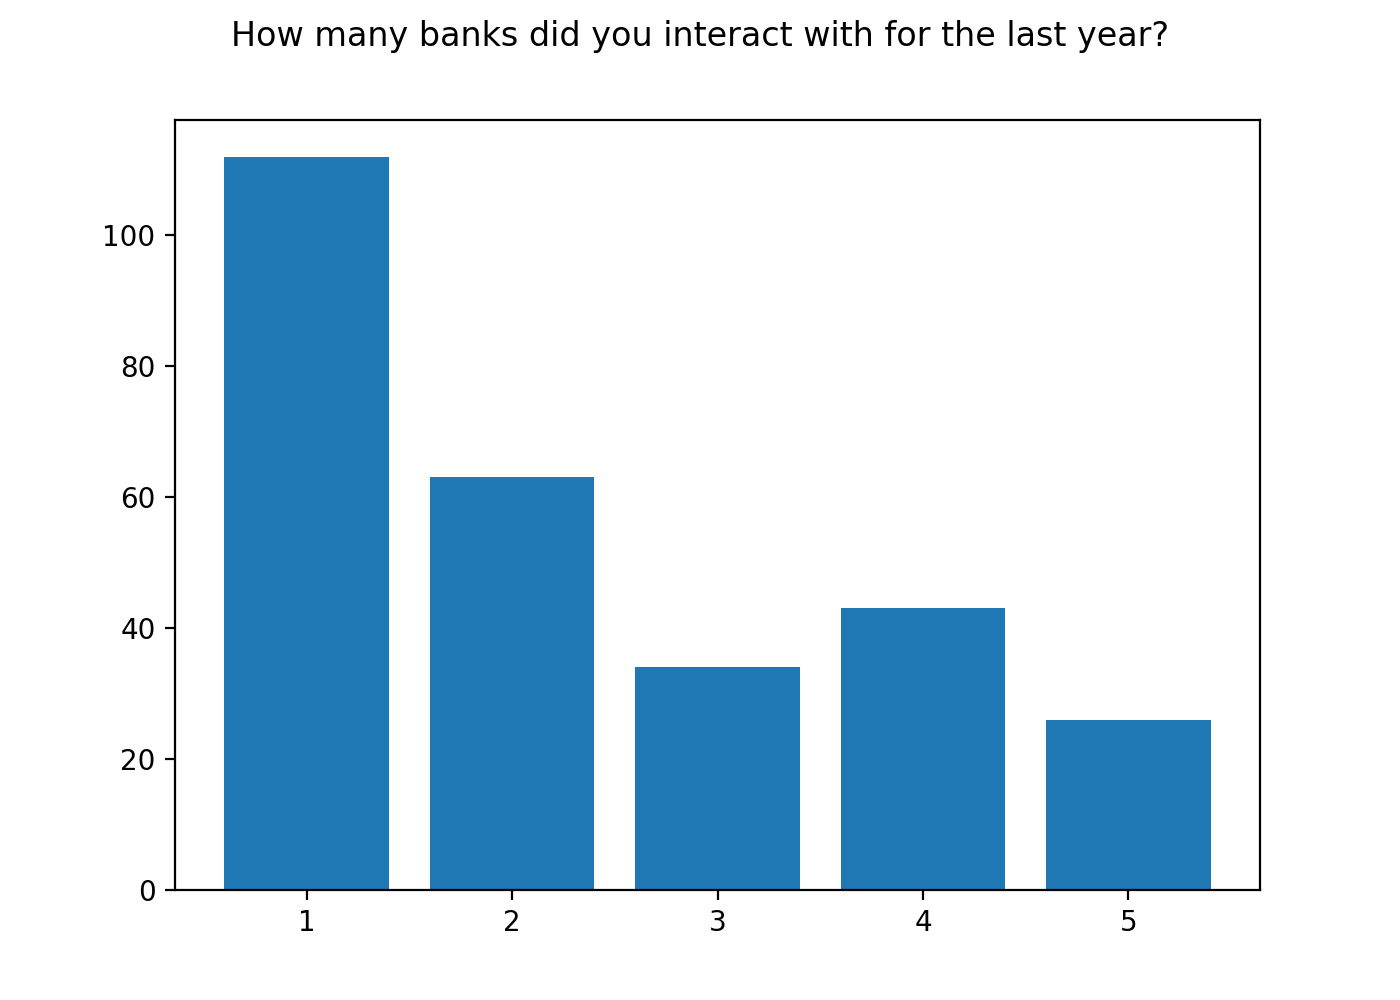
\includegraphics[width=0.6\textwidth,height=\textheight,keepaspectratio]{survey/2_how_many_banks_did_you_interact_with_for_the_last_year?.png}
    \caption{Number of banks per respondent}
    \medskip
    \footnotesize\textit{Source:} Own study.
\end{figure}

However, next two questions, question about satisfaction with banking interactions and question about satisfaction with problem-solving, had shown slightly negative feeling towards existing customer support systems.

\begin{figure}
    \centering
    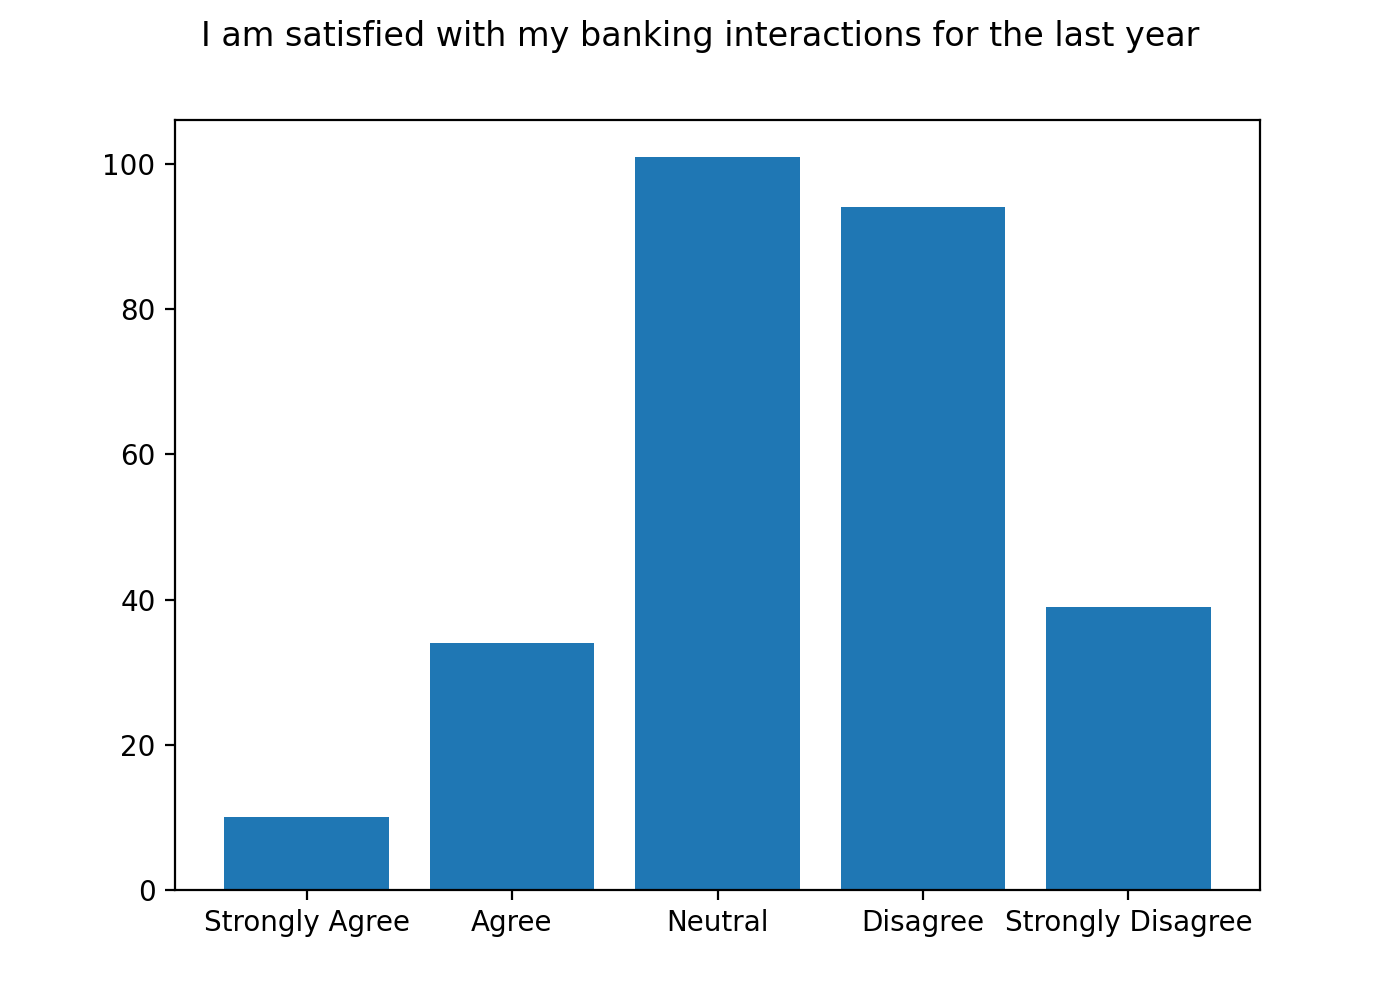
\includegraphics[width=0.6\textwidth,height=\textheight,keepaspectratio]{survey/3_i_am_satisfied_with_my_banking_interactions_for_the_last_year.png}
    \caption{Satisfaction with banking interaction}
    \medskip
    \footnotesize\textit{Source:} Own study.
\end{figure}

\begin{figure}
    \centering
    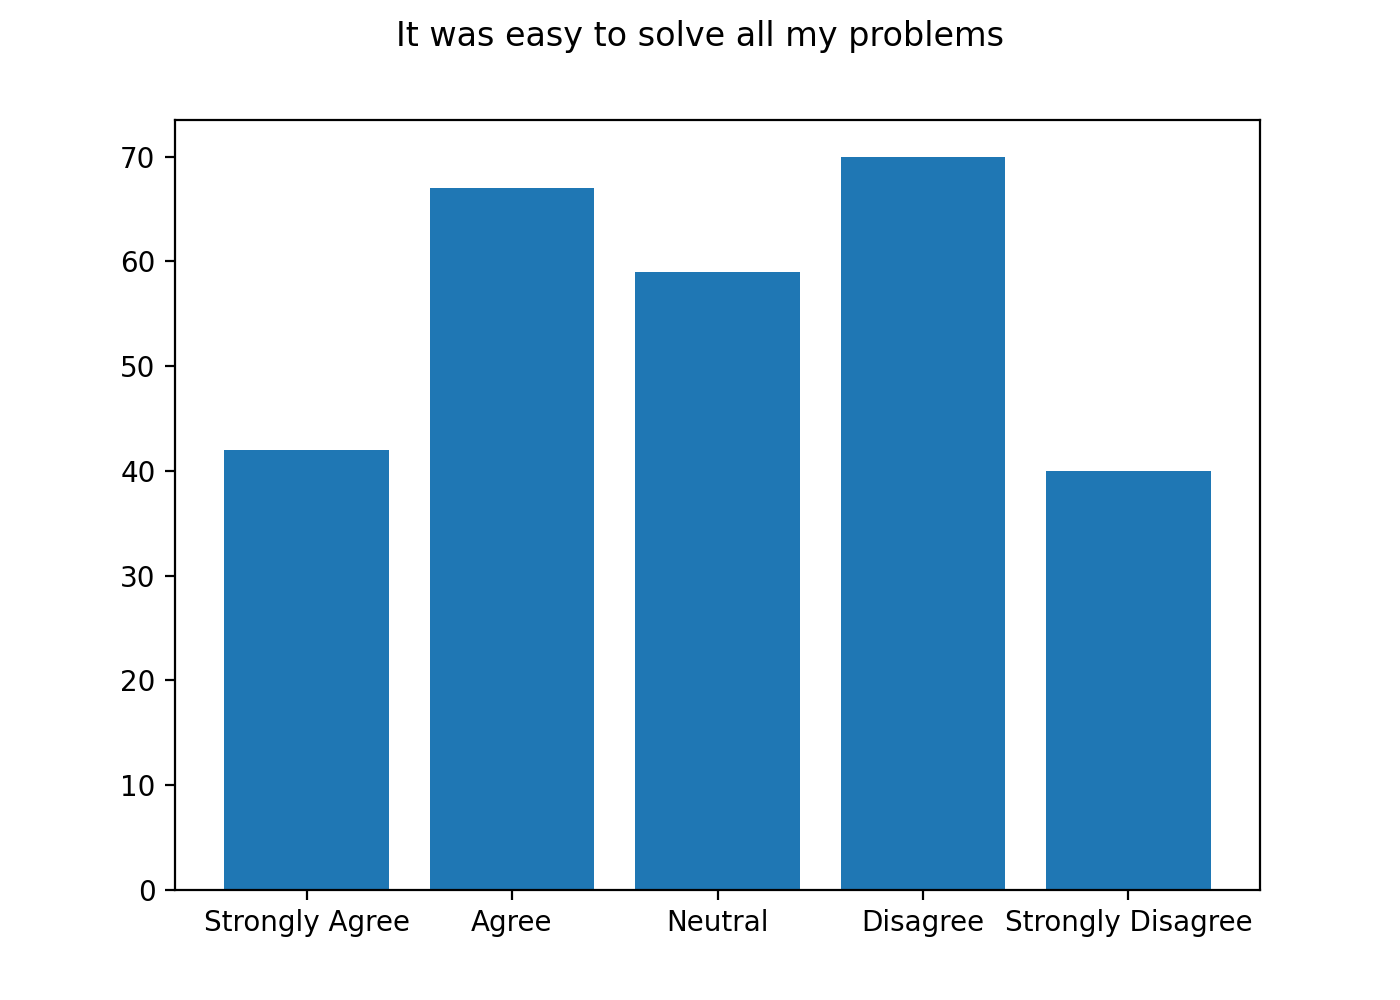
\includegraphics[width=0.6\textwidth,height=\textheight,keepaspectratio]{survey/4_it_was_easy_to_solve_all_my_problems.png}
    \caption{Satisfaction with problem-solving}
    \medskip
    \footnotesize\textit{Source:} Own study.
\end{figure}

At the same time, even though most of the researches had shown general dissatisfaction with response times, respondents of this survey were more loyal and showed neutrality.

\begin{figure}
    \centering
    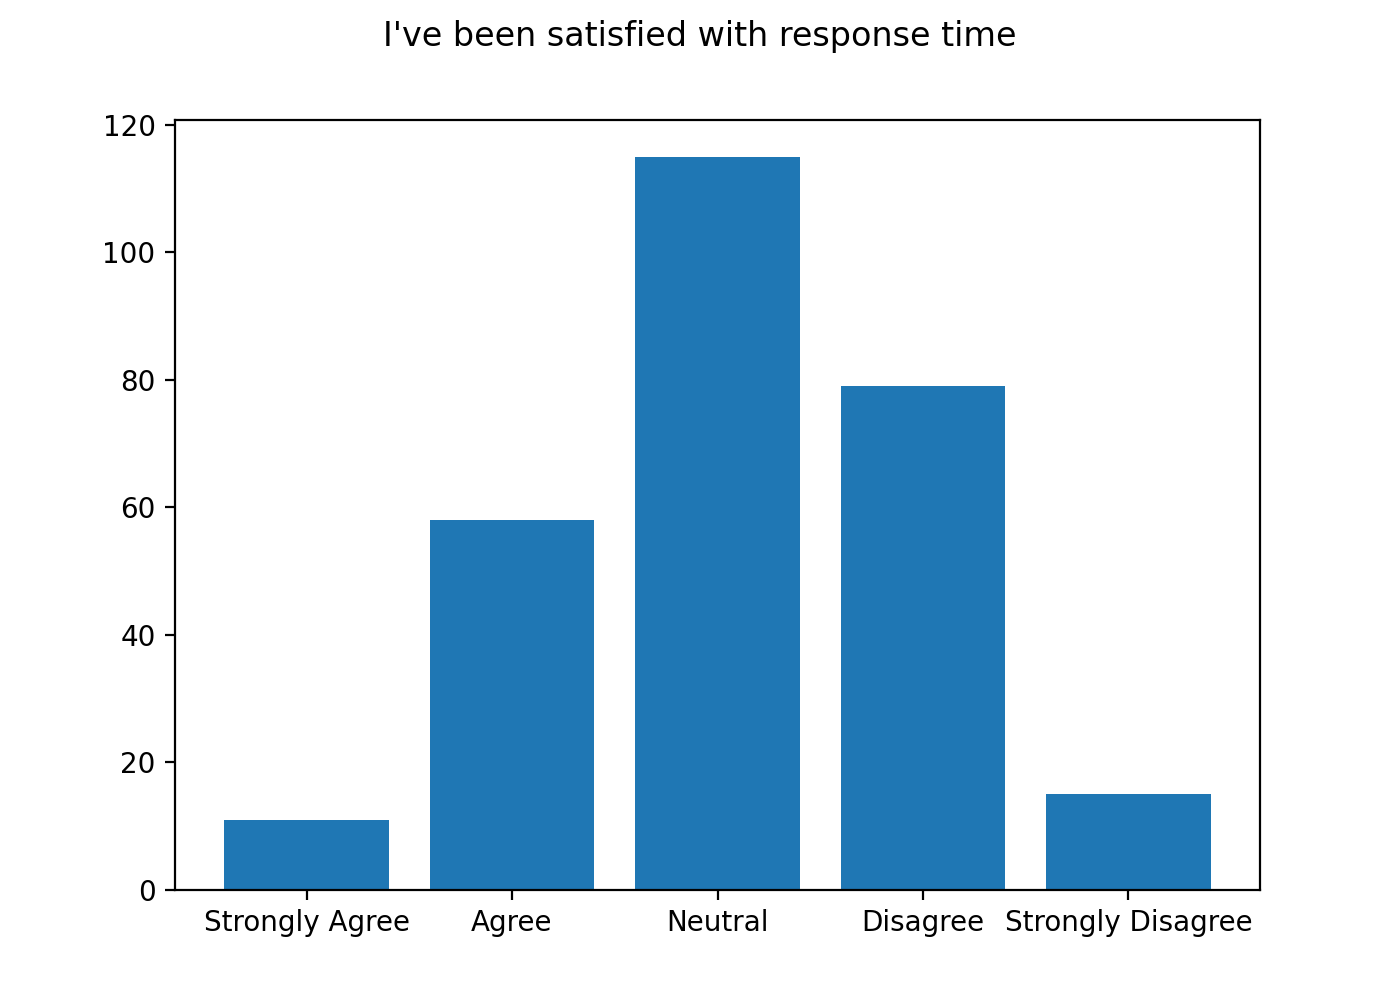
\includegraphics[width=0.6\textwidth,height=\textheight,keepaspectratio]{survey/5_i've_been_satisfied_with_response_time.png}
    \caption{Satisfaction with response time}
    \medskip
    \footnotesize\textit{Source:} Own study.
\end{figure}

Next question confirmed hypothesis about survey population and showed that respondents mostly prefer dialog interactions over phone calls.

\begin{figure}
    \centering
    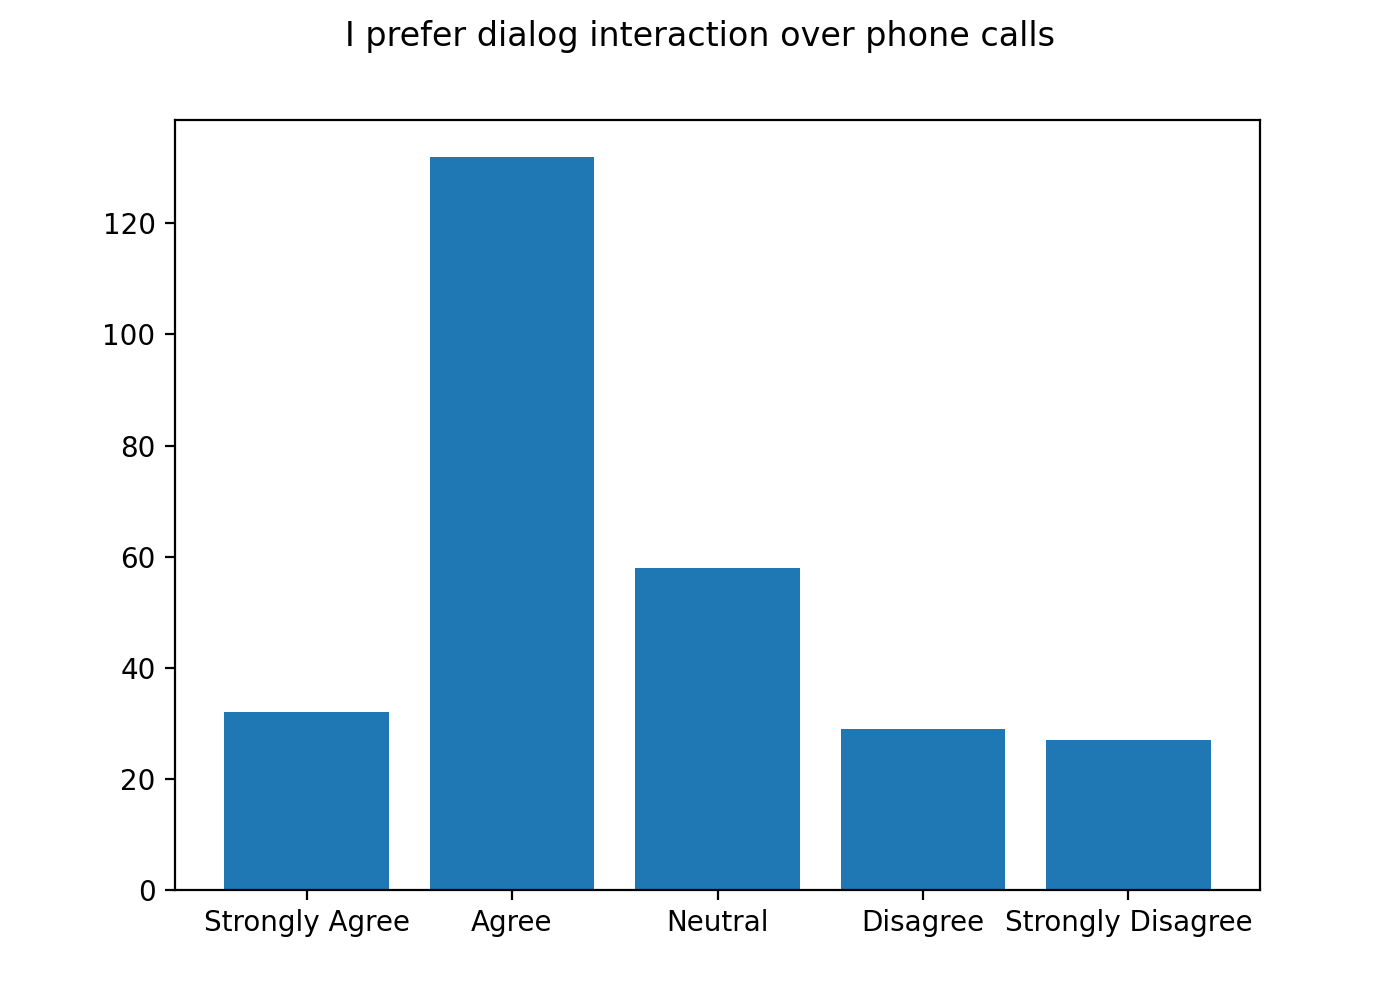
\includegraphics[width=0.6\textwidth,height=\textheight,keepaspectratio]{survey/6_i_prefer_dialog_interaction_over_phone_calls.png}
    \caption{Preferences between dialogs and calls}
    \medskip
    \footnotesize\textit{Source:} Own study.
\end{figure}

One of the most interesting results is high assurence of respondents that they know when they walk with a chat-bot, and not a human employee.

\begin{figure}
    \centering
    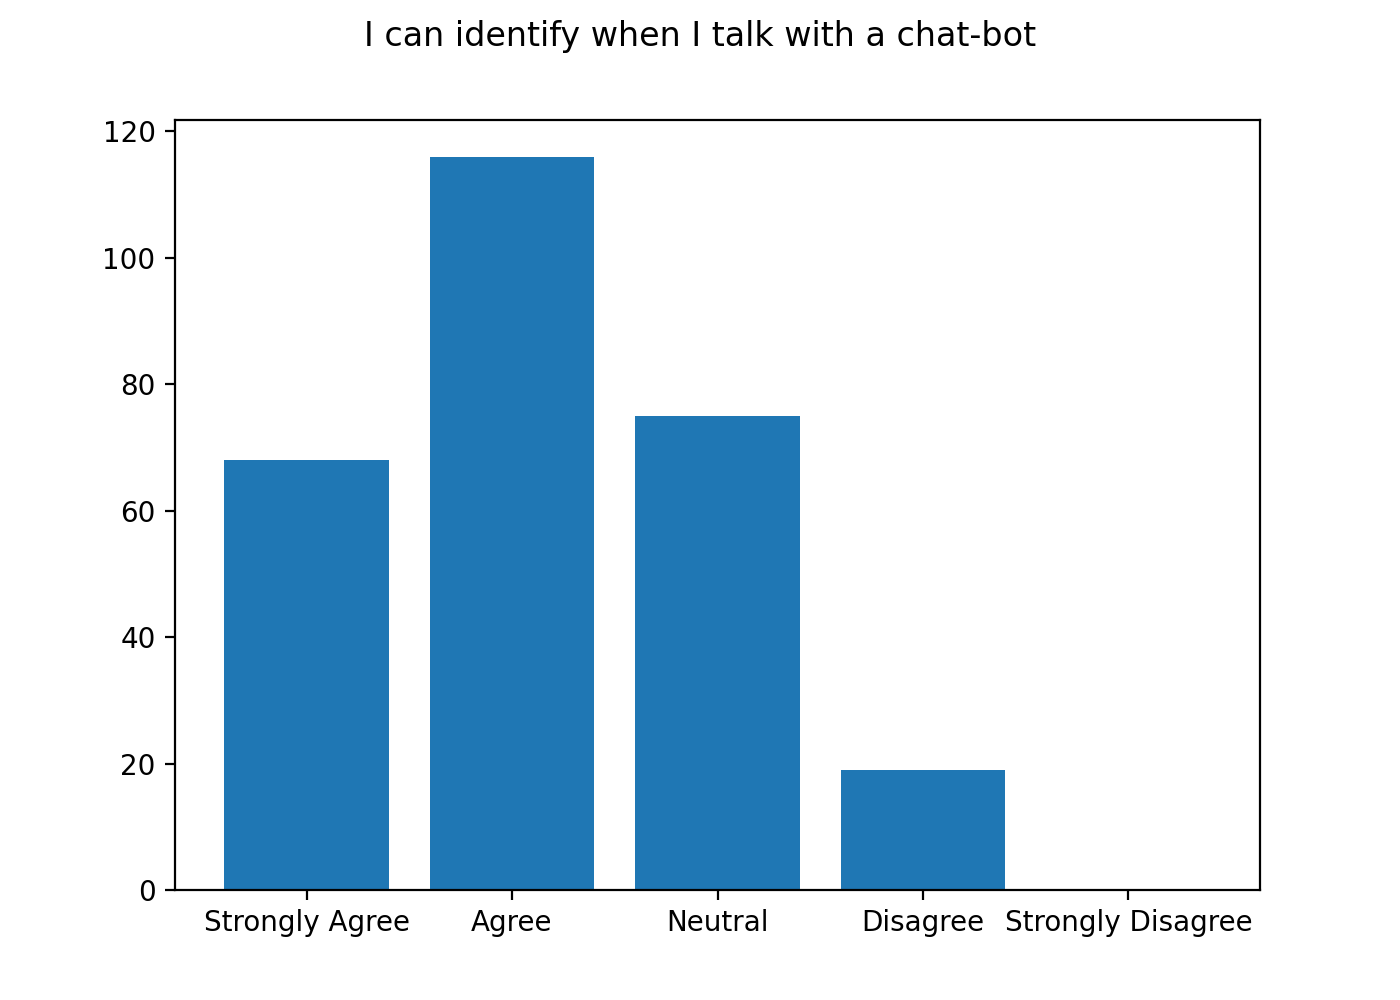
\includegraphics[width=0.6\textwidth,height=\textheight,keepaspectratio]{survey/7_i_can_identify_when_i_talk_with_a_chat-bot.png}
    \caption{Chat-bot awareness}
    \medskip
    \footnotesize\textit{Source:} Own study.
\end{figure}

However, I suspect this is connected to significant dissatisfaction with chat-bots, as there is a perfect negative correlation between questions about chat-bot awareness and satisfaction with chat-bots.

\begin{figure}
    \centering
    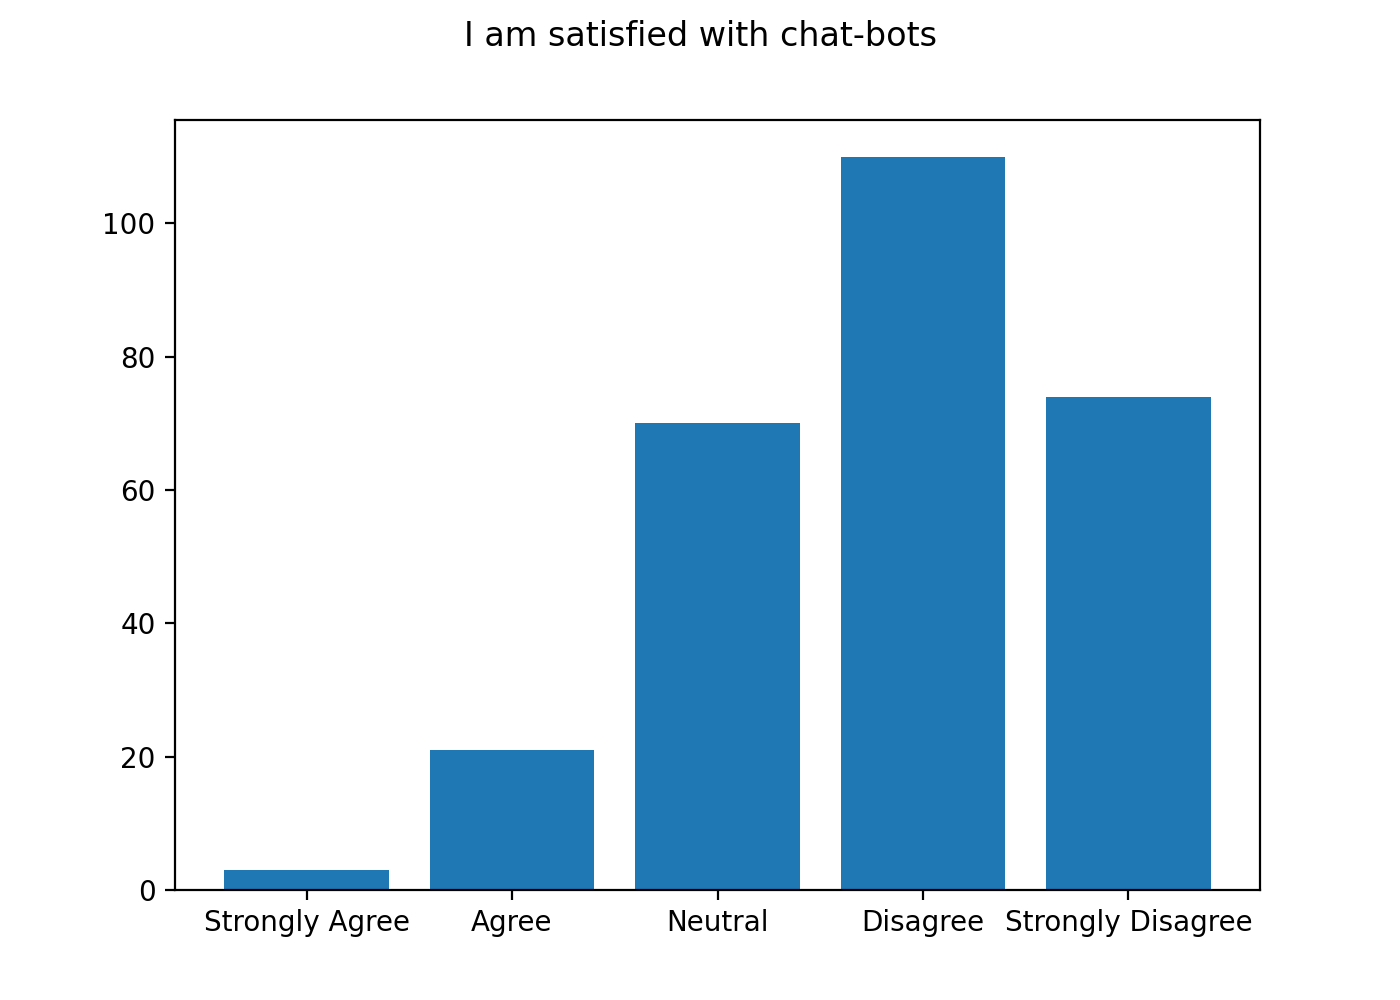
\includegraphics[width=0.6\textwidth,height=\textheight,keepaspectratio]{survey/8_i_am_satisfied_with_chat-bots.png}
    \caption{Satisfaction with chat-bot}
    \medskip
    \footnotesize\textit{Source:} Own study.
\end{figure}

Additionally, we can observe higher trust to human employees over automated solutions.

\begin{figure}
    \centering
    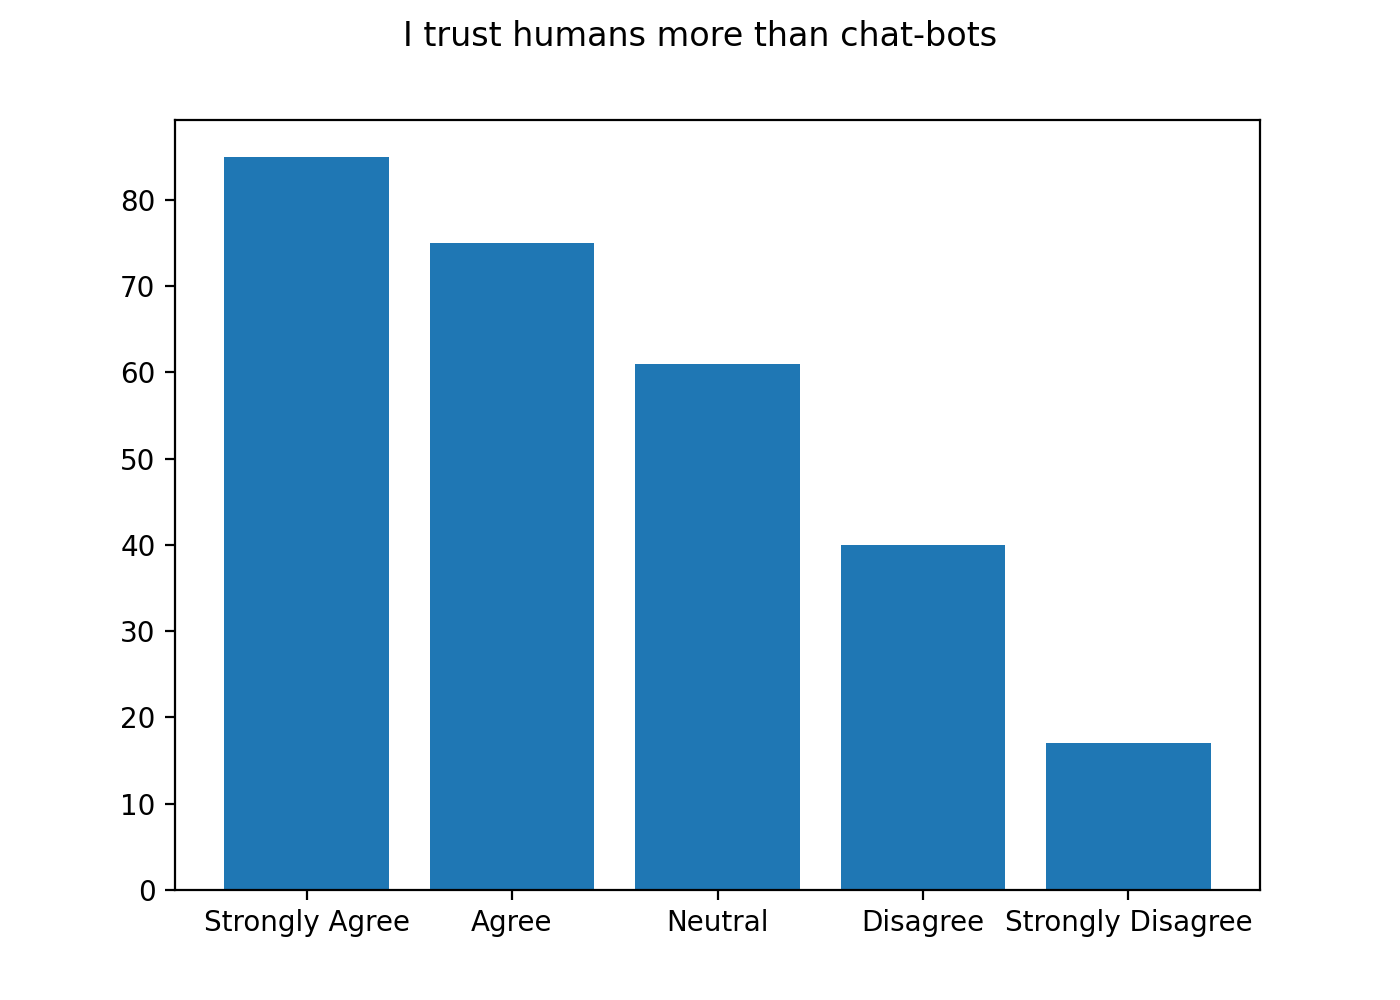
\includegraphics[width=0.6\textwidth,height=\textheight,keepaspectratio]{survey/9_i_trust_humans_more_than_chat-bots.png}
    \caption{Client trust towards interlocutor}
    \medskip
    \footnotesize\textit{Source:} Own study.
\end{figure}

As a result, survey showed a lot of interesting points and formed multiple conclusions.
In general, survey showed that people between 18 and 32 years old prefer dialog interfaces over vocal communication.
Moreover, clients will prefer dialog forms over other forms even though those are not as effective as clients expect and may result in slightly negative experience for client.
On the opposite, common argument of long response time may be outdated, as even more demanding generation of clients are neutral.

Although, dialogs are prefered, clients tend to trust people more.
In my opinion, this opinion is very subjective, as automated solutions may advise more exactly and don't require prior experience.
Probably, this is connected to high dissatisfaction with existing chat-bots effectiveness.
Moreover, negative impact of chat-bots forced clients to learn to determine when they talk to a chat-bot and when to an employee.
This results in a strong cleint association that chat-bots are bad and effective.

Consequently, next generation of chat-bots have to speak to clients in a natural language, in order to be indistinguishable from employee.
Thus, Artificial Intelligence technologies, including Machine Learning and Natural Language Programming are highly required.

Nevertheless, we can observe general minor satisfaction with existing form of user interaction and negative expectations about automated solutions.
This shows that clients are not ready for chat-bots yet.
Moreover, it is possible to conclude that chat-bots are not that much for consumers, as they are an important evolution milestone for the banks.

Even if there would be a chat-bot solution which passes some limited version of Turing test, when the customer finds
out that all that he was talking to a chat-bot, he may feel deceived and lost trust to a bank.

The main hypothesis of this thesis was that Commercial Banking clients are ready for Automated Front Offices in a form of Chat-bot with Artificial Intelligence and will positevely react to its injection into banking infrastracture.
Conclusively, this hypothesis has to be rejected.
People are not ready and have negative subjective feelings towards chat-bots.
Changing those feelings would require significant marketing costs.

However, the most valid injection of a chat-bot solution would be in a hybrid approach.
Hybrid approach is a synergy between human employee and an automated chat-bot system.
In hybrid approach robot recommends an answer to an operator based on existing knowledge base.
In this case, customer trusts and employee, but receives exact fast answer from an internal chat-bot system.